\documentclass{article}[10pt]

\usepackage{graphicx} % for pdf, bitmapped graphics files
\usepackage{epsfig} % for postscript graphics files
\usepackage{multirow}
\usepackage{fancyhdr}
%\usepackage{fullpage}
\usepackage{rotating}

\newcommand\T{\rule{0pt}{2.6ex}}
\newcommand\TT{\rule{0pt}{1.756ex}}
\newcommand\B{\rule[-1.2ex]{0pt}{0pt}}

%\pagestyle{fancy}

\setlength{\abovecaptionskip}{1ex}


\begin{document}

%\chead{This paper appeared in ICCD 2009 --- IEEE Copyright Rules Apply}

\title{\LARGE \bf
{\tt ll}: Exploring the Limits of Code Density
}

\author{ \parbox{3 in}{\centering Vincent M. Weaver\\
         \textit{University of Maine}\\
         {\tt vincent.weaver@maine.edu}}
}
%         \hspace*{0.5 in}
%         \parbox{3 in}{ \centering Sally A. McKee\\
%         \textit{Chalmers University of Technology}\\
%         \textit{mckee@chalmers.se}}
%}

\maketitle
%\thispagestyle{empty}
%\pagestyle{empty}

\begin{abstract}
This document is a continuation of my code density work as described
in our ICCD'09~\cite{weaver+:iccd09} paper.  
This is just a summary document meant to accompany the project sourcecode.  
Included are updated versions of the graphs and tables from the original
code density work, updated as new architectures are added.

I hand-assemble a simple benchmark on a number of architectures with
the end goal being the smallest code size.  
A comparison can then be made of the code density of the architecture.  
The benchmark is small and simple, so may not give a full accounting of 
code density for larger benchmarks, but picking a larger benchmark would 
make the hand-coded assembly task much larger.  
The benchmark does have some useful routines in it, such as 
LZSS compression~\cite{ziv+:lz77,storer+:lzss82}, 
string concatenation, and integer to string conversions.

\end{abstract}

\section{Additional Findings since ICCD'09}

In theory the new x86 SSE4 string instructions should be great for
doing some of these operations, such as strlen or strcat.
I could not find a way to use them to find the results in fewer
bytes than the discrete instructions.



\begin{figure}[tbp]
  \centering
  \epsfig{file=ll.eps,width=\columnwidth}
  \caption{Sample output from the {\tt linux\_logo} benchmark}
  \label{figure:ll}
\end{figure}

%
% Include the architecture table
%

\noindent
\begin{sidewaystable}[tbp]
\caption{Summary of investigated architectures}
\label{table:archtable}
\begin{sf}
\begin{footnotesize}
\begin{center}
\begin{tabular}{|c|c||c|c|c|c|c|c|c|c|c|c|c|}
\hline
\T \multirow{2}{*}{\bf Type} &
\multirow{2}{*}{\bf arch} &
\multirow{2}{*}{\bf endian$^{\star}$} & 
\multirow{2}{*}{\bf bits} & 
{\bf instr len} & 
{\bf op} & 
{\bf GP int} & 
{\bf unaligned} & 
{\bf auto-inc} & 
{\bf hw}  &
{\bf stat} &
{\bf branch} & 
{\bf predi-}\\

        & % Type
        & % arch
        & % Endian
        & % bits
{\bf (bytes)} & % instr len
{\bf args}    & % op
{\bf regs}    & % GP int
{\bf ld/st}   & % unaligned
{\bf address} & % auto-inc
{\bf div}     & % HW
{\bf flags}   & % stat
{\bf delay}   & % branch 
{\bf cation}\\  % predi-

\hline\hline

%%%%%%%%%%%%%%%%%%%%%%%%%%%%%%%%%%%%%%%%%%%%%%%%% VLIW

\multirow{1}{*}{\bf VLIW} &
% IA64
IA64             &  % ARCH  
%VLIW             &  % TYPE
%2001		    % year
little           &  % endian 
64               &  % bits
16/3$^{\dagger}$ &  % instr length
3                &  % arguments 
127,zero         &  % GP int regs
no               &  % unaligned accesses 
yes              &  % auto-inc
no               &  % hw-divide
yes              &  % status flags  
no               &  % branch delay slot
yes                 % predication
\\
\hline
\hline

%%%%%%%%%%%%%%%%%%%%%%%%%%%%%%%%%%%%%%%%%%%%%%%%%%%% RISC

\multirow{8}{*}{\bf RISC} &
% Alpha
Alpha            & % ARCH
%RISC            & % Type
%1992		 & % Year
little           & % endian
64               & % bits 
4                & % instr length
3                & % arguments
31, zero         & % GP int regs
no               & % unaligned accesses
no               & % auto-inc
no               & % hw-divide 
no               & % status flags
no               & % branch delay slot
no                 % predication
\\
\cline{2-13}

% ARM
                 & % Type
ARM              & % ARCH
%RISC             & % Type
%1986		 & % Year
little           & % endian
32               & % bits
4                & % instr-length
3                & % arguments
15,PC            & % GP int regs
no               & % unaligned accesses
yes              & % auto-inc
no               & % HW divide
yes              & % status flags
no               & % branch delay slot
yes                % predication
\\
\cline{2-13}

% m88k
		 & % Type
m88k             & % ARCH
%RISC            & % Type
%1988		 & % Year
big              & % endian
32               & % bits
4                & % instr-length
3                & % arguments
31,zero          & % GP int regs
no               & % unaligned accesses
no               & % auto-inc
Q only           & % HW divide
no               & % status flags
optional         & % branch delay slot
no                 % predication
\\
\cline{2-13}

% microblaze
		 & % Type
MicroBlaze       & % ARCH
%RISC            & % Type
%2001?		 & % Year
big              & % endian
32               & % bits
4                & % instr-length
3                & % arguments
31,zero          & % GP int regs
no               & % unaligned accesses
no               & % auto-inc
Q only$^{\star\star}$ & % hw-divide
no               & % status flags
optional         & % branch delay slot
no                 % predication
\\
\cline{2-13}

% MIPS
		 & % Type
MIPS             & % ARCH
%RISC            & % Type
%1985		 & % Year
big              & % endian
32/64            & % bits
4                & % instr-length
3                & % arguments
31,hi/lo,zero    & % GP int regs
yes$^{\star\star}$& % unaligned accesses
no               & % auto-inc
yes              & % hw-divide
no               & % status flags
yes              & % branch delay slot
no                 % predication
\\
\cline{2-13}

% PA-RISC
                 & % Type
PA-RISC          & % ARCH
%RISC            & % Type
%1989		 & % Year
big              & % endian
32/64            & % bits
4                & % instr-length
3                & % arguments
31,zero          & % GP int regs
no               & % unaligned accesses
no               & % auto-inc
part             & % hw-divide
no               & % status flags
yes              & % branch delay slot
no                 % predication
\\
\cline{2-13}

% PPC
                 & % Type
PPC              & % ARCH
%RISC            & % Type
%1991		 & % Year
big              & % endian
32/64            & % bits
4                & % instr-length
3                & % arguments
32               & % GP int regs
yes              & % unaligned accesses
yes              & % auto-inc
Q only           & % HW divide
yes              & % status flags
no               & % branch delay slot
no                 % predication
\\
\cline{2-13}

% RiSC
                 & % Type
RiSC             & % ARCH
%RISC            & % type
%1998		 & % Year
big              & % endian
16               & % bits
2                & % instr-length
3                & % arguments
7,zero           & % GP int regs
no               & % unaligned accesses
no               & % auto-inc
no               & % hw divide
no               & % status flags
no               & % branch delay slot
no                 % predication
\\
\cline{2-13}

% SPARC
                 & % Type
SPARC            & % ARCH
%RISC            & % Type
%1985		 & % Year
big              & % endian
32/64            & % bits
4                & % instr-length
3                & % arguments
63-527,zero$^{\ddagger}$ & % GP int regs
no               & % unaligned accesses
no               & % auto-inc
Q only           & % hw-divide
yes              & % status flags
yes              & % branch delay slot
no                 % predication
\\

\hline\hline

%%%%%%%%%%%%%%%%%%%%%%%%%%%%%%%%%%%%%%%%%%%%%%% CISC

\multirow{5}{*}{\bf CISC} &
% m68k
m68k             & % ARCH
%CISC            & % type
%1979		 & % Year
big              & % endian
32               & % bits
2-22             & % instr-length
2                & % arguments
16               & % GP int regs
yes              & % unaligned accesses
yes              & % auto-inc
yes              & % hw divide
yes              & % status flags
no               & % branch delay slot
no                 % predication
\\
\cline{2-13}

% s390
		 & % Type
s390             & % ARCH
%CISC            & % Type
%1964		 & % Year
big              & % endian
32/64            & % bits
2-6              & % instr-length
2                & % arguments
16               & % GP int regs
yes              & % unaligned accesses
no               & % auto-inc
yes              & % hw divide
yes              & % status flags
no               & % branch delay slot
no                 % predication
\\
\cline{2-13}

% VAX
                 & % Type
VAX              & % ARCH
%CISC            & % type
%1977		 & % Year
big              & % endian
32               & % bits
1-54             & % instr-length
3                & % arguments
16               & % GP int regs
yes              & % unaligned accesses
yes              & % auto-inc
yes              & % hw divide
yes              & % status flags
no               & % branch delay slot
no                 % predication
\\
\cline{2-13}

% x86
                 & % Type
x86              & % ARCH
%CISC            & % type
%1978		 & % Year
little           & % endian
32               & % bits
1-15             & % instr-length
2                & % arguments
8                & % GP int regs
yes              & % unaligned accesses
yes              & % auto-inc
yes              & % hw divide
yes              & % status flags
no               & % branch delay slot
no                 % predication
\\
\cline{2-13}

% x86_64
		 & % TYPE
x86\_64          & % ARCH
%CISC            & % Type
%2000		 & % Year
little           & % endian
32/64            & % bits
1-15             & % instr-length
2                & % arguments
16               & % GP int regs
yes              & % unaligned accesses
yes              & % auto-inc
yes              & % hw divide
yes              & % status flags
no               & % branch delay slot
no                 % predication
\\

\hline\hline

%%%%%%%%%%%%%%%%%%%%%%%%%%%%%%%%%%%%%%%%%%%%%%%%%%%%%% Embedded

% avr32
\multirow{4}{*}{\bf Embedded} &
AVR32            & % ARCH
%embed           & % type
%2006		 & % Year
big              & % endian
32               & % bits
2                & % instr-length
2                & % arguments
15,PC            & % GP int regs
yes              & % unaligned accesses
yes              & % auto-inc
yes              & % hw divide
yes              & % status flags
no               & % branch delay slot
no                 % predication
\\
\cline{2-13}

% CRISv32
                 & % Type
CRISv32          & % ARCH
%embed           & % type
%2000		 & % Year
little           & % endian
32               & % bits
2-6              & % instr-length
2                & % arguments
16,zero,special  & % GP int regs
yes              & % unaligned accesses
yes              & % auto-inc
part             & % hw divide
yes              & % status flags
yes              & % branch delay slot
no                 % predication
\\
\cline{2-13}

% SH3
                 & % Type
SH3              & % ARCH
%embed           & % type
%1992		 & % Year
little           & % endian
32               & % bits
2                & % instr-length
2                & % arguments
16,MAC           & % GP int regs
no               & % unaligned accesses
yes              & % auto-inc
part             & % hw divide
yes              & % status flags
yes              & % branch delay slot
no                 % predication
\\
\cline{2-13}

% THUMB
                 & % Thumb
THUMB            & % ARCH
%embed           & % type
%1995		 & % Year
little           & % endian
32               & % bits
2                & % instr-length
2                & % arguments
8/15,PC          & % GP int regs
no               & % unaligned accesses
no               & % auto-inc
no               & % hw divide
yes              & % status flags
no               & % branch delay slot
no                 % predication
\\
\cline{2-13}

% THUMB-2
                 & % Thumb
THUMB-2          & % ARCH
%embed           & % type
%1995		 & % Year
little           & % endian
32               & % bits
2-4              & % instr-length
2-3              & % arguments
8/15,PC          & % GP int regs
no               & % unaligned accesses
yes              & % auto-inc
no               & % hw divide
yes              & % status flags
no               & % branch delay slot
yes                % predication
\\
\cline{2-13}


\hline
\hline
%%%%%%%%%%%%%%%%%%%%%%%%%%%%%%%%%%%%%%%%%%%%%%%% 8/16-bit

% 6502
\multirow{3}{*}{\bf 8/16-bit} &
6502             & % ARCH
%8-bit           & % Type
%1975		 & % Year
little           & % endian
8                & % bits
1-3              & % instr-length
1                & % arguments
3                & % GP int regs
yes              & % unaligned accesses
no               & % auto-inc
no               & % hw-divide
yes              & % status flags
no               & % branch delay slot
no                 % predication
\\
\cline{2-13}

% 8086
                 & % Type
8086             & % ARCH
%16-bit          & % type
%1978		 & % Year
little           & % endian
16               & % bits
1-15             & % instr-length
2                & % arguments
8                & % Gp int regs
yes              & % unaligned accesses
yes              & % auto-inc
yes 		 & % hw-divide
yes              & % status flags
no               & % branch delay slot
no                 % predication
\\
\cline{2-13}

% pdp-11
                 & % Type
PDP-11           & % ARCH
%16-bit          & % type
%1970		 & % Year
little           & % endian
16               & % bits
2-6              & % instr-length
2                & % arguments
6,sp,pc          & % Gp int regs
no               & % unaligned accesses
yes              & % auto-inc
yes$^{\star\star}$& % hw-divide
yes              & % status flags
no               & % branch delay slot
no                 % predication
\\
\cline{2-13}

% z80
                 & % Type
z80              & % ARCH
%8-bit           & % type
%1976		 & % Year
little           & % endian
8                & % bits
1-4              & % instr-length
2                & % arguments
18               & % Gp int regs
no               & % unaligned accesses
lim              & % auto-inc
no 		 & % hw-divide
yes              & % status flags
no               & % branch delay slot
no                 % predication
\\
\cline{2-13}

\hline

\end{tabular}

$^{\star}$ on the machine we used \hspace{2em}$^{\dagger}$ 16-byte bundle has 3 instructions
\hspace{3em}$^{\ddagger}$ register windows, only 32 visible
\hspace{2em}$^{\star\star}$ many implementations
\end{center}
\end{footnotesize}
\end{sf}
\end{sidewaystable}
% Longest intel instruction?  Some claim 17, longest I could find is 15
%15 [16-bit]
%66 67 F0 3E 81 04 4E 01234567 89ABCDEF
%add [ds:esi+ecx*2+0x67452301], 0xEFCDAB89
%13 [32-bit]
%F0 3E 81 04 4E 01234567 89ABCDEF
%lock add [ds:esi+ecx*2+0x67452301], 0xEFCDAB89
% 15 [64-bit]
%F0 65 67 4c 81 84 80 01234567 89abcdef
% lock:add qw gs:Zpg[EAX+RD8*4+67452301h],-10325477h 
% VAX POLYG can be 56 bytes.  Or is it 54?


% Include Correlations Table
\begin{table}[tbp]
\caption{Correlations of architectural features to binary size}
\label{table:correlations}
\begin{sf} 
\begin{center}
\begin{tabular}{|r@{.\hspace{0.025em}}l|l|}
\hline
\multicolumn{2}{|c|}{\bf Correlation} & \multirow{2}{*}{\bf Architectural Parameter}\\
\multicolumn{2}{|c|}{\bf Coefficient} & \\
\hline
\hline
 0 & 9381 	& Minimum possible instruction length \\
 0 & 9116	& Number of integer registers \\
 0 & 7823       & Virtual address of first instruction \\ 
 0 & 6607	& Architecture has a zero register \\
 0 & 6159	& Bit-width \\
 0 & 4982	& Number of operands in each instruction \\
 0 & 3129	& Year the architecture was introduced \\
 \hline
-0 & 0021	& Branch delay slot \\
-0 & 0809	& Machine is big-endian \\
-0 & 2121	& Auto-incrementing addressing scheme \\
-0 & 2521	& Hardware status flags (zero/overflow/etc.) \\
-0 & 3653	& Unaligned load/store available \\
-0 & 3854	& Hardware divide in ALU \\
\hline
\end{tabular}
\end{center}
\end{sf}
% 0.6160	& Predicated instructions \\
% 0.0126	& Maximum possible instruction size  \\
%
% Explain
%   Positive correlation means high val of feature increases code size 
%   Negative correlation means high val of feature decreased code size
\end{table}


% Figure on total code size
\begin{figure}[tbp]
  \centering
  \epsfig{file=ll_total_size.eps,width=\textwidth}
  \caption{Total size of benchmarks 
           (includes some platform-specific code, so does not
           strictly reflect code density)}
  \label{figure:total}
\end{figure}

% Decompression Code
\begin{figure}[tbp]
  \centering
  \epsfig{file=ll_lzss_size,width=\textwidth}
  \caption{Size of LZSS decompression code}
  \label{figure:decomp}
\end{figure}

% String concatenation code
\begin{figure}[tbp]
  \centering
  \epsfig{file=ll_strcat_size,width=\textwidth}
  \caption{Size of string concatenation code (machines with 
           auto-increment addressing modes and dedicated
           string instructions perform better). 6502 behaves poorly as it
           lacks an increment-16-bit-register instruction.}
  \label{figure:strcat}
\end{figure}

% Findstring code
\begin{figure}[tbp]
  \centering
  \epsfig{file=ll_findstring_size,width=\textwidth}
  \caption{Size of string searching code (unaligned load
           instructions help, since four bytes at arbitrary offsets 
           can be compared at once.  
           CISC architectures as well as avr32 and MIPS benefit)}
  \label{figure:findstring}
\end{figure}

% Integer printing code
\begin{figure}[tbp]
  \centering
  \epsfig{file=ll_num_ascii.eps,width=\textwidth}
  \caption{Size of integer printing code (hardware
           divide helps code density)}
  \label{figure:numascii}
\end{figure}

% LibC Sizes
\begin{figure}[tbp]
  \centering
  \epsfig{file=libc_sizes.eps,width=\textwidth}
  \caption{Size comparison}
  \label{figure:libc}
\end{figure}

\pagebreak

{
\bibliographystyle{plain}
\bibliography{ll_document}
}


\end{document}
